%\chapter{Design}
%\label{chap:design}
%
%
%In this chapter we introduce a first approach of a visual formalism and later state the final desing of the visual language. Furthermore the idea of automated constraint generation is presented in section~\ref{sec:automatedconstraintgeneration}. The assembly of all the previous features in one tool is described in section~\ref{sec:coalescence}. However, the tool's functionality shall also be available in Robostudio in order to provide safety mechanisms for the healthcare service robots. Section~\ref{sec:integrationintorobostudio} gives a main idea how an integration into Robostudio ought to be. 
%
%%The challenge now is to find a similar intuitive and nonmathematical way of representing reasonable safety constraints for the healthbot domain and to figure out how to translate it to corresponding textual expressions. The new concept will be integrated into Robostudio, a design tool for statemachines, in order to enable the user to create safety constraints visually. A common LTL model checker will be added to it as well which fulfils the verification of the translated constraints on the designed statemachine. In case of verification failures the concerning constraints and a visual counter example can be presented.




\chapter{Visual formalisms}
\label{chap:visualformalisms}

In this chapter we introduce two different approaches of visual formalisms and later state the final desing of the visual language.
One main difficulty in finding a proper visual formalism is to glean the right level between abstraction and expressiveness since this two characteristics appear to be mutually exclusive in some points. A first approach, so called template constraints and its pros and cons are described in section~\ref{sec:templateconstraints}. Subsequently an improved design is presented, which tends to a more abstract direction.




\section{Template constraints}
\label{sec:templateconstraints}

%It is not a trivial issue to find a
What visual presentation of constraints would suit a healthbot application developer and what are the main types of safety constraints he could want to check?
% TODO: wir haben gedacht, dass es einfach zu benutzen ist
Leaded by this question, we developed a visual language based on templates. These templates make different propositions about states and their relations. The user can choose from several graphical constraint types and customize them by parameterizing state variables. So far there are two different kinds of template constraints:

\begin{enumerate}
	\item Whenever state (x) is active, state (y) must be visited before state (z) can be reached.
	
	The idea behind this constraint is, that propositions about temporal dependencies can be made. Under certain circumstances a visit of a particular state is restricted as long as a specific precondition is fulfilled. Example of a constraint: Whenever a person is eating (x), he must brush his teeth (y) before he can go to bed (z). Going to bed without brushing teeth after meal should never happen.
	\item Each visit of state (x) will eventually result in a visit of either state (y) or state (z) [or state (w) [...]]. All of them are actually reachable.
	
	This constraint type enforces at least one particular event to happen after a spezific precondition.
	Example of a constraint: Every time a person enters a supermarket (x) he will eventually decide to buy 
	%a product or not to buy it.
	something (y) or to leave the shop with empty hands (z). He finally has to make a decision, but he can't avoid both possibilities.
	Nitpicking readers might note the person could also steel something without buying it, and thus not buy anything but leave the shop with full hands. Of course this is true; exactly in this case our constraint would signal an undesirable "program" behavior with its invalidity.
\end{enumerate}

Figure~\ref{fig:templateconstraints} gives a visual suggestion how the two constraint types could look like. Each state of a constraint is symbolized by the robot surface to make the user think he's directly working with the robot. Furthermore the state labels should sometimes be replaced by the screen displays of the regarding states. All parameters of the template constraints can be customized by just clicking on one robot suface. In the subsequently appearing popup window (figure~\ref{fig:templateconstraint_dropdown}) all states contained in the underlying program are listed and can be chosen.
 
\begin{figure}[htbp]
  \centering
  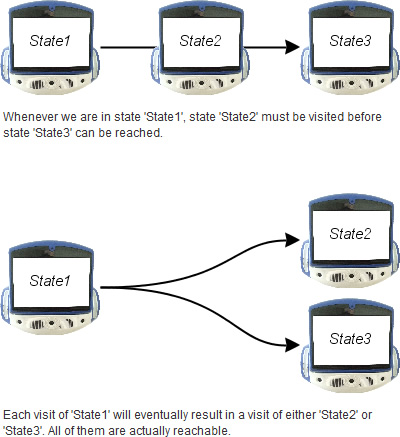
\includegraphics[scale=0.7]{templateconstraints}
  \caption{The two template constraint types, parameterized with particular states.}
  \label{fig:templateconstraints}
\end{figure}

\begin{figure}[htbp]
  \centering
  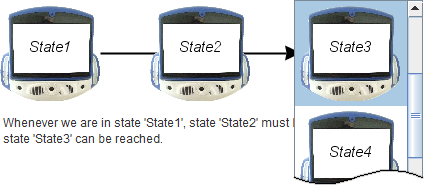
\includegraphics[scale=0.7]{templateconstraint_dropdown}
  \caption{Dropdown menu for spezifying template parameter.}
  \label{fig:templateconstraint_dropdown}
\end{figure}

This visual language was presented to potential users for evaluation and feedbak. Though most of them named it a good concept, soon it turned out that there are some problems and disagreements. The presented constraints were interpreted differently, the semantic seemd to be unclear and not unique.
A try to solve this problem was to equip both constraint templates with textual explanations which are updated automatically whenever there is a change in parameterization. These additional expressions are also shown in figure~\ref{fig:templateconstraints}.
But unfortunately even the textual eplanations don't seem to be a satisfying solution. For example, one question came up whether the first constraint template allows state (x) to be visited more than once before state (z) is reached.

However, there is a second lack with the template constraints.
Whereas lots of safety constraints specific to the healthcare domain mentioned in section~\ref{sec:healthbotapplication} are expressable by this visual language, there are a lot of other common constraints which have no matching template and thus can't be described. Not even the check of a state being visited never or at least once is possible. This lack of expressiveness appears to be too big and for this reason the approach of template constraints got dismissed.

%idee: einfache verwendung
%sehr spezialisiert auf healthcare anwendung







\section{Operator constraints}
\label{sec:operatorconstraints}

With our second approach we try to gain more expressiveness and uniqueness for the visual language. For this we decided to decrease the abstraction level and design a visual formalism for linear temporal logic (LTL, see~section~\ref{sec:modelcheckingandltl}). Since the visual constraints can be directly mapped to LTL expressions, the visual language is equal to LTL in expressiveness. If it is considered as easy to use, two birds get killed with one stone: Non-experts can use it as well as experts.

% Gefundene probleme, die man erw�hnen k�nnte: beim if operator ist das �bergeordnete always nicht intuitiv. der always operator k�nnte umgedreht sein. 

%The presented visual language is designed to express constraints for state machines.
To provide the required functionality, the fundamental logical operators are required, as shown in (a) though (e) below. In addition the visual language should be capable of expressing constraints about future steps, both (h) any future state and (g) the next state, that (f) events should always happen, and that (i) a property must be true until some future event. Like in Del Bimbo et al.'s formula representation~\cite{520786}, a constraint consists of nested operators and propositions in a hierarchy. However we surrender the three dimensional idea and focus on two dimensional blocks and their compositions instead, what is also used by HomeTL~\cite{4341725}.
Each block represents either an operator or a proposition and has its specified semantics. Thus a visual formula can be recursively translated to a linear temporal logic (LTL) sentence and be checked using any ordinary model checker. 

The visual language has support for eight operator types and one proposition as shown in figure~\ref{fig:operators}. 

\begin{description}
	\item[(a)] \emph{AND} operator: $\varphi \wedge \psi$.
	\item[(b)] \emph{OR} Operator: $\varphi \vee \psi$.
	\item[(c)] \emph{IF} operator: $\varphi \Rightarrow \psi$.\\Instead of an \emph{IMPLIES} operator an \emph{IF} operator is provided. Its meaning seems to be more intuitive for non-experts since it is a common construct in almost every programming language.
	\item[(d)] \emph{NOT} operator: $\neg \varphi$.
	\item[(e)] Proposition: $\rho$.\\Until now there is only the \emph{state proposition} type, which gives evidence about the currently active state. Other types such as numeric or string equations may be added but are less important for our healthcare subject.
	\item[(f)] \emph{ALWAYS} operator: $\Box \varphi$.\\$\varphi$ must be true now and in all following states.
	%\Box \Diamond \medcircle
	\item[(g)] \emph{NEXT} operator: $\medcircle \varphi$.\\$\varphi$ has to be true in the next state.
	\item[(h)] \emph{FUTURE} operator: $\Diamond \varphi$.\\At least one time - now or in a later state - $\varphi$ must be true.
	\item[(i)] \emph{UNTIL} operator: $[\varphi \mathcal{U} \psi]$.\\Now and in all following states $\varphi$ must be true until there is a state with $\psi$ being true. In addition eventually there has to be a future state with $\psi$ being true.
\end{description}


\begin{figure}[htbp]
  \centering
  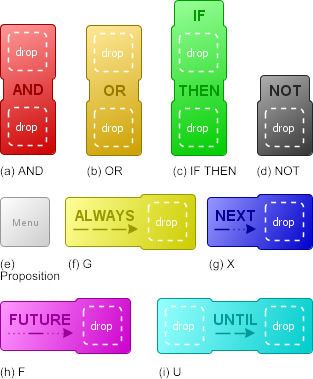
\includegraphics[scale=0.65]{table}
  \caption{The visual language consists of eight unary or binary operator types and one state proposition, each of them having its own color flavor. Logical operators are arranged in a vertical row wereas time relevant statements are aligned horizontally.}
  \label{fig:operators}
\end{figure}



To meet the requirements the visual language should be very easy to use, especially for non-experts. Furthermore it should provide an intuitive application which is ideally learnable within little time. So there are some design decisions this visual language must fulfill~\cite{moody-physics-of-notations}:

\begin{itemize}
	\item Each operator has a different significant visual appearance; in this case we have used color. This kind of classification enables a faster subconscious identification.
	\item The layout of constraints (nested operators) has two dimensions with a certain meaning. Figure~\ref{fig:directions} demonstrates the ``logical'' vertical read direction as well as the time releveant horizontal line.
	\item Multiple nested operators of the same kind which have no order priorities such as \emph{OR} or \emph{AND} appear unnecessarily complex. These operators can be merged (see~figure~\ref{fig:nested_and}).
\end{itemize}

\begin{figure}[htbp]
  \centering
  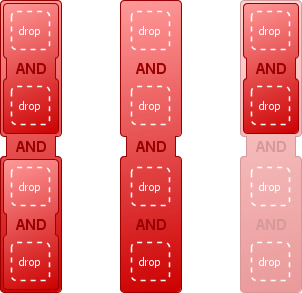
\includegraphics[scale=0.65]{and_simplify} %width=0.7\linewidth
  \caption{In order to simplify the appearance of constraints certain operators might be merged. Merged nested \emph{AND} operators (center) are less complex as default ones (left). However nested \emph{AND} operators with mouse over (right) are displayed separated in order to retain full editability.}
  \label{fig:nested_and}
\end{figure}

Also an editor for this visual language can contribute to usability and clarity. Some requirements are as follows:

\begin{itemize}	
	\item All editing is performed only by simple drag and drop. Operators and propositions can be moved and dropped onto other operators. A tool bar provides all operator and proposition types to be instantiated and there is a trash can for deleting existing operators.
	\item In order to simplify the reading of constraints an operator can be hovered over by the mouse pointer. All higher operators become bleached out so that the hovered operator and its children appear highlighted. It's intended to be similar to line coloring when reading a digital text.
	\item Every edit to either the constraint or the underlying state machine results in an automatically (re-)validation of the constraint. The result is immediately displayed to the user.
	\item There are different statuses which inform about validation result: For syntactically invalid constraints, an ``incomplete'' sign is displayed. Otherwise, an animated ring indicates that validation is in pro\-gress and will finally result in either a ``valid'' or ``invalid'' sign (see~figure~\ref{fig:results}).
	\item There is no button for constraint creation / editing except operator and proposition providers, which let the developer create new instances. Having no additional buttons reduces complexity and keeps it simple.
\end{itemize}


\begin{figure}[htbp]
  \centering
  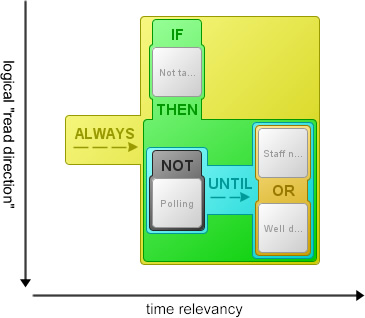
\includegraphics[scale=0.65]{directions}
  \caption{Easy understanding of visual constraints due to intuitive read directions: ``ALWAYS is true: IF state \emph{'Not taken yet'} is active THEN state \emph{'Polling'} can NOT be visited UNTIL state \emph{'Staff notified'} OR state \emph{'Well done!'} is reached.''}
  \label{fig:directions}
\end{figure}

\begin{figure}[htbp]
  \centering
  
\includegraphics[scale=0.65]{results}
  \caption{Status indicators displaying validation results: incomplete, validation in pro\-gress, invalid and valid.}
  \label{fig:results}
\end{figure}





\chapter{Automated constraint generation}
\label{chap:automatedconstraintgeneration}

As already mentioned before, it might be difficult for developers to find all reasonable safety constraints by hand which are needed for full safety covery. Hence it also can happen, that a prior software version was correct and over time mistakes crept in because of minor adjustments once in a while.
To help prevent this to happen, we introduce the concept of automated constraint generation for state machines. Once a program reaches a complete condition, constraint suggestions which are valid on the current program can be computed fully automatically. On the one hand they may help the developer identifying reasonable constraints he didn't think about as well as contradictions between program and specification, eg. if a computed constraint doesn't make sense at all. On the other hand all constraints can be revalidated after each change to the software and thus ensure consistency.

In order to support the developer in developing safe programs, automated generation and suggestion of constraints might be helpful. But it's helpful only if the suggested constraints are relevant and reasonable.


\section{Subgraph definition}
\label{sec:subgraphdefinition}

Whether suggested constraints are relevant and reasonable
%This however
depends on the domain and use case. It has to be mentioned that our approach of finding an algorithm for constraint finding presented in this work has a special focus on the healtcare use cases and may not be applicable for other domains.
Regarding the important constraints postulated in chapter~\ref{chap:goals}, we found out that all all the relevant states fall into one of the following categories:

\begin{enumerate}
	\item States having two or more outgoing transitions ($\alpha$-states).
	\item States in which all paths starting from one $\alpha$-state come together again ($\beta$-states).
	\item All States immediately before $\beta$ states ($\gamma$-states).
\end{enumerate}

In order to compute the required constraints automatically, and possibly additional ones, we deal with subgraphs defined as follows:
%Um die in requirements definierten constraints und vielleicht noch mehr zu finden, behelfen wir uns 
%Each $\alpha$-, the corresponding $\beta$- and several $\gamma$-states form a part of a state set called \emph{subgraph}. In order to retreive valid constraints a subgraph is defined by the following requirements: %as follows

\begin{itemize}
	\item There is a start state ($\alpha$-state) with at least two outgoing transitions.
	\item There is one end state ($\beta$-state) in which all possible paths starting from start state come together again.
	\item All states between the start and end states have no other incoming transitions than the ones originally coming from the start state. That means there is no path to visit these states except through the start state.
	\item The start state may have incoming transitions from states not contained in the subgraph.
	\item The end state may have incoming and outgoing transitions from and to states not contained in the subgraph.
\end{itemize}


\begin{figure}[htbp]
  \centering
  
  \tikzstyle{state} = [circle,fill=white,draw]
  \tikzstyle{statein} = [circle,fill=blue!20,draw]
  \tikzstyle{every path} = [font=\sffamily\small]
  
	\begin{tikzpicture}[->,>=stealth',shorten >=1pt,auto,node distance=15mm]
	
	
%	  \node[statein] (1) {$\alpha$};
%	  \node[state] (2) [above left of=1] {};
%	  \node[state] (3) [below left of=1] {};
%	  \node[statein] (4) [above right of=1] {};
%	  \node[statein] (5) [below right of=1] {};
%	  \node[statein] (8) [right of=5] {$\gamma$};
%	  \node[statein] (6) [right of=4] {$\gamma$};
%	  \node[statein] (7) [below right of=4] {$\gamma$};
%	  
%	  \node[statein] (9) [right of=7] {$\beta$};
%	  \node[state] (10) [above of=9] {};
%	  \node[state] (11) [above right of=9] {};
%	  \node[state] (12) [below right of=9] {};
%	  
%	  \path[dashed]
%	    (2) edge node [left] {} (1)
%	    (3) edge node [left] {} (1)
%	    (10) edge node [left] {} (9)
%	    (9) edge node [left] {} (11)
%	    (9) edge node [left] {} (12);
%		\path[]
%	  	(1) edge node [left] {} (4)
%	        edge node [left] {} (5)
%	    (4) edge node [left] {} (6)
%	        edge node [left] {} (7)
%	    (5) edge node [left] {} (8)
%	    (6) edge node [left] {} (9)
%	    (7) edge node [left] {} (9)
%	    (8) edge node [left] {} (9)
%	    ;
	    
	    
	  \node[statein] (1) {$\alpha$};
	  \node[state] (2) [above left of=1] {};
	  \node[state] (3) [above right of=1] {};
	  \node[statein] (4) [below left of=1] {};
	  \node[statein] (6) [below of=4] {$\gamma$};
	  \node[statein] (7) [below right of=4] {$\gamma$};
	  \node[statein] (5) [below right of=1] {};
	  \node[statein] (8) [below of=5] {$\gamma$};
	  \node[statein] (9) [below of=7] {$\beta$};
	  \node[state] (10) [right of=9] {};
	  \node[state] (11) [below left of=9] {};
	  \node[state] (12) [below right of=9] {};
	  
	  \path[dashed]
	    (2) edge node [left] {} (1)
	    (3) edge node [left] {} (1)
	    (10) edge node [left] {} (9)
	    (9) edge node [left] {} (11)
	    (9) edge node [left] {} (12);
		\path[]
	  	(1) edge node [left] {} (4)
	        edge node [left] {} (5)
	    (4) edge node [left] {} (6)
	        edge node [left] {} (7)
	    (5) edge node [left] {} (8)
	    (6) edge node [left] {} (9)
	    (7) edge node [left] {} (9)
	    (8) edge node [left] {} (9)
	    ;
	
	\end{tikzpicture}
  \caption{Example for a subgraph.}
  \label{fig:subgraph}
\end{figure}

A graphical example of such a subgraph is shown in Fig.~\ref{fig:subgraph}. Using this specification all possible such subgraphs can be detected within a state machine.



\section{Constraint determination}

If the subgraph contains neither inner (infinite) loops nor final states (states having no outgoing transition) we can derive the following valid LTL formulas for each subgraph (with $\alpha$ as proposition for ``$\alpha$ is current state'' and similarly for $\beta$ and $\gamma$):

\begin{equation} \label{eq:first}
  \models \Box (\alpha \Rightarrow \Diamond \beta)
\end{equation}

\begin{equation} \label{eq:second}
  \models \Box (\alpha \Rightarrow \Diamond (\bigvee_{\gamma} \gamma))
\end{equation}

\begin{equation} \label{eq:third}
  \models \Box (\alpha \Rightarrow [\neg \beta \mathcal{U} \bigvee_{\gamma} \gamma])
\end{equation}

Additionally, for all states not contained in the subgraph (let's call them $\delta$-states, and the proposition $\delta$ stands for ``$\delta$ is current state'') the following formula is true: 

\begin{equation} \label{eq:fourth}
  \models \Box (\alpha \Rightarrow [(\bigwedge_{\delta} \neg \delta) \mathcal{U} \beta])
\end{equation}

In case of $\alpha = \beta$ - i.e. when all paths starting from $\alpha$-state eventually return again (cycle) - even another constraint can be assumed to be true:

\begin{equation} \label{eq:fifth}
  \models \Box \Diamond \alpha
\end{equation}
 

These five constraints apply to each subgraph matching the conditions mentioned above. Formula~\ref{eq:first} says that an $\alpha$-state is always eventually followed by a $\beta$-state. Formula~\ref{eq:second} ensures that there will be always at least one $\gamma$-state be visited after each visit of an $\alpha$-state. The quite similar but stricter formula~\ref{eq:third} demands additionally a visit of at least one $\gamma$-state before the $\beta$-state can be reached. Formula~\ref{eq:fourth} simply says that a state not contained in the subgraph can't be visited between $\alpha$- and $\beta$-states. The constraint that the $\alpha$-state will always eventually be visited again is expressed by formula~\ref{eq:fifth}.

All formulas can be translated to the visual formalism presented in section~\ref{sec:operatorconstraints} and shown to the user. The appropriate LTL formulas for the constraints postulated in chapter~\ref{chap:goals} relate to number \ref{eq:second} and \ref{eq:fifth} of the subgraph based formula templates and are as follows:

\begin{equation}
  \models \Box \Diamond \textnormal{'Polling'}
\end{equation}

\begin{equation}
	\models \Box (\textnormal{'Not taken yet'} \Rightarrow \Diamond (\textnormal{'Well done!'} \vee \textnormal{'Staff notified'})
\end{equation}
%	\item The program will always eventually check the database for new reminder jobs. Thus we avoid that pending reminder are never processed.
%	\item Either a reminded medication is taken properly or caregivers get notified whenever a patient refuses medication intake.